\graphicspath{{chapters/chapter2/}}
\chapter{State of the Art} \label{chapter2}
\section{Medical background}
\label{7ptSection}
%%%
\subsection{Skin Lesion}
A \textbf{skin lesion} is a part of the skin that has particular differences from the surrounding skin; the American Society for Dermatologic Surgery described it as an abnormal lump, bump, ulcer, sore, or colored area of the skin.
There are different types of skin lesion which differ in their characteristics such as shape, surface, colour, structure which could change overtime (See Figures \ref{fig:MEL_images} and \ref{fig:NEV_images} for an example) \\
Figure~\ref{fig:NEV_images} shows one of the most common skin lesions in the population, a Nevus. \textbf{Nevus}, also called mole, is a growth on the skin that develops when pigment cells (melanocytes) grow in clusters.  Nevus is harmless, and rarely can turn into skin cancer. \\
Skin lesions can be temporary or permanent depending on the causes, and most of them, as nevi, are harmless, but some can be warnings of skin cancer.\\
Skin cancer is the most common malignancy in fairskinned populations, and the incidences of melanoma and non-melanoma skin cancers are rising \cite{7ptCNNforMel}.
There are three common types of skin cancers: squamous cell carcinoma(SCC), basal cell carcinoma(BCC) and \textbf{melanoma}. The first two are tipically grouped together as non melanoma skin cancer, while malignant Melanoma (Figure~\ref{fig:MEL_images}) is a type of skin cancer which tends to spread to the other parts of the body causing death if is not diagnosed early \cite{7ptCNNforMel}\\
Early melanoma diagnosis showed to reverse the odds in the majority of cases \cite{mtl7ptCoppola}.
Wrong diagnosis  could cause death, especially when melanomas have a non-alarming clinical appearance and imitate a completely benign lesion. Against that, dermatologists nowadays are adopting innovative tools such as the dermatoscope for the acquisition of clearer images for an accurate diagnosis. Such tools along with particular rules and methods have allowed efficient identification of the early phase of cutaneous malignant melanoma.\\

\begin{figure}
    \centering
    \begin{subfigure}[b]{0.48\linewidth}        %% or \columnwidth
        \centering
        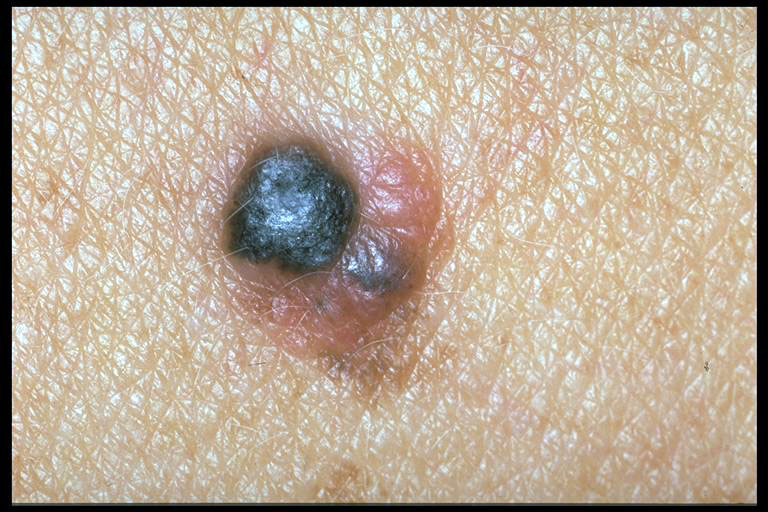
\includegraphics[width=\linewidth]{images/skin lesion/MEL/Gcl051.jpg}
        \caption{Clinical image\footnotemark[1]}
        
        \label{fig:Mel_A}
    \end{subfigure}
    \begin{subfigure}[b]{0.48\linewidth}        %% or \columnwidth
        \centering
        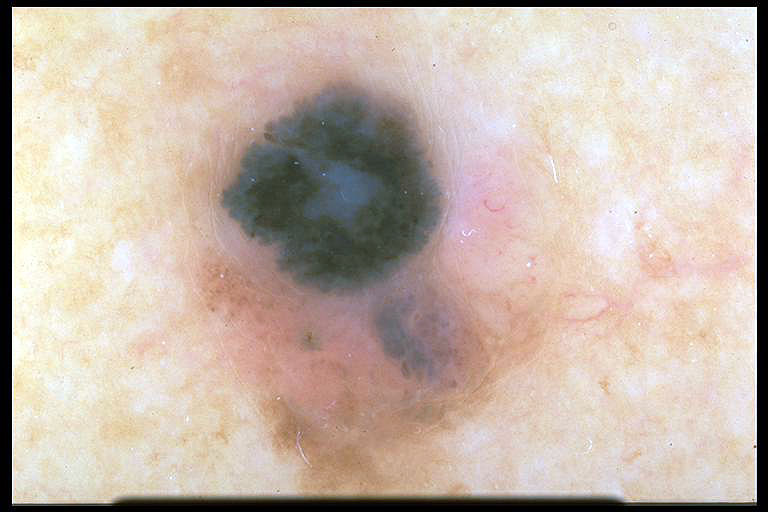
\includegraphics[width=\linewidth]{images/skin lesion/MEL/Gcl052.jpg}
        \caption{Dermatoscopy image\footnotemark[2]}
        \label{fig:Mel_B}
    \end{subfigure}
    \caption*{Source: https://derm.cs.sfu.ca/Welcome.html}
    \caption{Melanoma (more than 1.5 mm) with typical pigment network(7-point score: 0), irregular streaks (score: 1), diffuse irregular pigmentation (score: 1), absent regression structures(score : 0), irregular dots and globules (score : 1), present blue whitish veil (score : 2), irregular vascular structures(score : 2). Seven-point total score: 7
    }
 
    \label{fig:MEL_images}
\end{figure}


\subsection{Dermoscopy}
\textbf{Dermoscopy} is a noninvasive method that allows,  with a handheld instrument called Dermatoscope, the in vivo evaluation of colors and microstructures that are not visible to the naked eye \cite{Dermoscopy}. It features a light source and a magnifier and works a little like a magnifying glass.
Dermoscopy allows recognizing patterns and through appropriate techniques allows to determine the final diagnosis(See Figures \ref{fig:Mel_B} and \ref{fig:nev_B} for an example of Dermatoscopy images).\\ 

\footnotetext[1]{Clinical image: image acquired without dermatoscope}
\footnotetext[2]{Dermatoscopy image: image acquired with dermatoscope}

\subsection{Skin lesion classification techniques}
The most common techniques for skin cancer recognition are the ABCDE rule and the 7-point checklist.
Both techniques have been developed to simplify the diagnostic process based on pattern analysis, used to differentiate benign from malignant skin tumours. \\ \\
To help to identify characteristics of unusual moles that may indicate melanomas or other skin cancers,  \textbf{ABCDE rule} consists of, looking for:
\begin{enumerate}[label=(\Alph*)]
\item asymmetrical shape. Look for moles with irregular shapes, such as two very different-looking halves.
\item irregular border. Look for moles with irregular, notched or scalloped borders - characteristics of melanomas.
\item changes in color. Look for growths that have many colors or an uneven distribution of color.
\item diameter. Look for new growth in a mole larger than 1/4 inch (about 6 millimeters).
\item evolving. Look for changes over time, such as a mole that grows in size or that changes color or shape. Moles may also evolve to develop new signs and symptoms, such as new itchiness or bleeding.
\end{enumerate}

\begin{figure}
    \centering
    \begin{subfigure}[b]{0.48\linewidth}        %% or \columnwidth
        \centering
        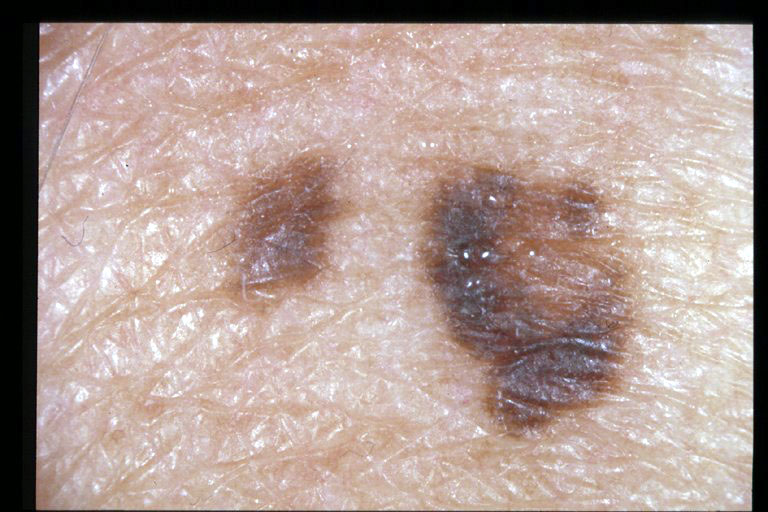
\includegraphics[width=\linewidth]{images/skin lesion/NEV/Aal005.jpg}
        \caption{Clinical image}
        \label{fig:nev_A}
    \end{subfigure}
    \begin{subfigure}[b]{0.48\linewidth}        %% or \columnwidth
        \centering
        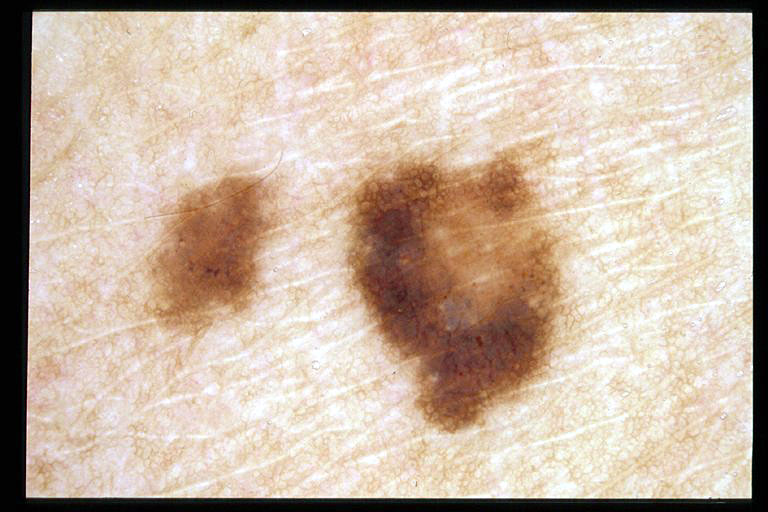
\includegraphics[width=\linewidth]{images/skin lesion/NEV/Aal006.jpg}
        
        \caption{Dermatoscopy  image}
        \label{fig:nev_B}
    \end{subfigure}
    \caption*{Source: https://derm.cs.sfu.ca/Welcome.html}
    \caption{Clark nevus with typical pigment network(7-point score: 0), absent streaks (score: 0), diffuse irregular pigmentation(score: 1), blue areas regression structures(score : 1), regular dots and globules (score : 0), absent blue whitish veil (score : 0), absent vascular structures(score : 0). Seven-point total score: 2}

    \label{fig:NEV_images}
\end{figure}
Cancerous (malignant) moles vary greatly in appearance. Some may show all of the changes listed above, while others may have only one or two unusual characteristics\cite{melanoma1}. \\ \\
\label{7ptRule}
The \textbf{Seven Point Checklist} was established by Argenziano et al.~\cite{Derm7ptData} for the dermoscopic differentiation between benign melanocytic lesions and melanoma. 
The dermoscopic evaluation,the 7-Point Check List, proceeds by calculating a score according to a scoring system, in which each tally is  assigned by evaluating irregular and atypical pattern, as shown in Table~\ref{table:1}.\\
A score equal to or greater than 3 predisposes to the diagnosis of melanoma (for practical example of the scoring system see Figures \ref{fig:MEL_images} and \ref{fig:NEV_images}).\\
This criteria is a widely used diagnostic method in the diagnosis of melanoma. Cutaneous malignancies can be identified with some certainty through this analytical procedure. All recognized melanomas have at least one of the seven main criteria defined by this system.
Numerous studies have confirmed the sensitivity of this method in the diagnosis of melanoma such as in \cite{7ptGeneralPractice}.
Its practicality consists in providing a public awareness of the visible characteristics of the tumor and thus shortening the waiting times for a specialized medical consultation and to ensure timely and appropriate intervention by the general doctor.


\begin{table}[]
\begin{tabular}{ |p{12cm}|p{0.8cm}|}
 \hline
 \multicolumn{2}{|c|}{\textbf{7-Point Score criteria}} \\
 \hline
 Dermoscopic pattern & Score \\
 \hline
 \textbf{Atypical network:} Combination of at least two types of pigment network (in terms of colour and thickness of the lines) asymmetrically distributed within the lesion & +2\\
 \textbf{Blue-white veil:} Irregular, structureless area of confluent blue pigmentation with an overlying white ‘ground-glass’ film. The pigmentation cannot occupy the entire lesion and usually corresponds to a clinically elevated part of the lesion & +2\\
 \textbf{Atypical vascular pattern:} Linear-irregular vessels, dotted vessels and/or milky-red areas not clearly seen within regression structures & +2 \\
\textbf{Irregular dots/globules:} More than three round to oval structures, brown or black in colour, asymmetrically distributed within the lesion & +1 \\
\textbf{Irregular streaks:} More than three brown to black, bulbous or finger-like projections asymmetrically distributed at the edge of the lesion and not clearly arising from network structures & +1 \\
\textbf{Irregular blotches:} Black, brown and ⁄or grey structureless areas asymmetrically distributed within the lesion & +1 \\
\textbf{Regression structures:} White scar-like depigmentation and/or blue pepper-like granules usually corresponding to a clinically flat part of the lesion & +1 \\
\hline
\end{tabular}
\caption{Dermoscopic criteria and scoring system of the classic version of the ‘seven-point checklist’ dermoscopic algorithm}
\label{table:1}
\end{table}
\clearpage
\section{Technical background}
\textbf{Deep neural networks}(DNN) mimic the human mind by replicating millions of connections between neurons, and basically consist of multiple layers interconnected through single units, the neurons. Depending on the inputs received, a neuron can be activated or not, producing a signal that is sent to another neuron on a hidden layer. This process continues until the signal has propagated to the output layer.
\subsection{Neurons}
Neurons are the building blocks of neural networks.
\begin{figure}[b]
    \centering
        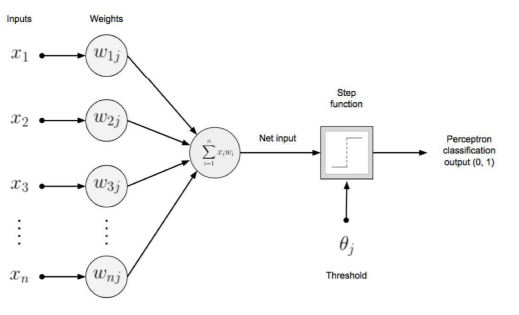
\includegraphics[width=0.7\linewidth]{images/deepLearning/neural block.png}
    \caption{Neuron structure \cite{DeepLearningApproach} }
    \label{fig:Neuron}
\end{figure}\\
Figure \ref{fig:Neuron} shows one of the basic structures of a neuron. A set of inputs are weighed and summed. The result is then used as an input for an activation function that determines how much the neuron will be activated by the signal received as an input. In the image:
\begin{enumerate}
    \item $x_i$ is the i-th input value.
    \item $w_i$ is the weight applied to $x_i$.
    \item $\theta$ is the activation threshold.
\end{enumerate}
The activation function is just a rule to determine how much will be activated; there are different types of activation functions, among which, the most common are the Sigmoid Function and the Relu Activation Function.\\
Sigmoid activation function produces an output in the range [0,1] while the ReLu produces $max(0,x)$ as output.
\subsection{Networks}
A neural network is made up of many neurons organized in layers. The figure shows a simple example of a neural network.
\begin{figure}[ht]
    \centering
        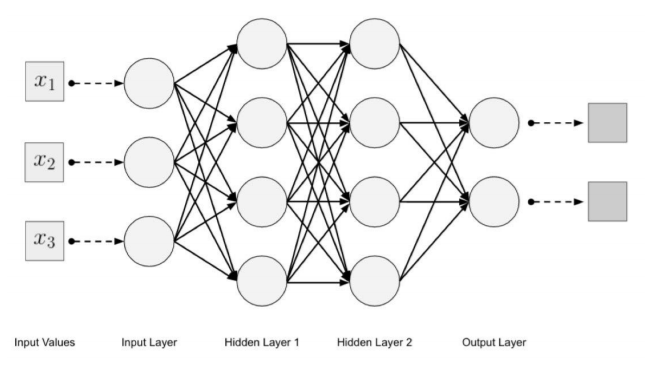
\includegraphics[width=0.7\linewidth]{images/deepLearning/network.png}
    \caption{Neural Network structure \cite{DeepLearningApproach} }
    \label{fig:Network}
\end{figure}
These types of networks use fully-connected layers which forward their outputs to all neurons in the next layer.
Each internal layer is called hidden layer. The output layer produces a set of relative probability values, related to a class. Typically, the final layer is a softmax, which converts the output of the previous one into a probability distribution.
\\ \\
The most common way to train a DNN is by supervising the training. Supervised learning is performed by using a set of input paired with the corresponding label output.
The network tries to mimic the training set, by modifying the network parameters during each training epoch, in order to reduce the value of a function, called cost function, which expresses the difference between the current output and the ground truth.
\\\\
The main common characteristic of deep learning methods is their focus on feature learning: automatically learning representations of data. Discovering features and performing a task is merged into one problem, and therefore both improve during the same training process \cite{deepLearningMRIimaging}.
Recently, deep learning has become one of the most successful techniques and achieved impressive performance in the computer vision field.
\textbf{Image classification} is the task of assigning an input image one label from a fixed set of categories. This is one of the core problems in Computer Vision that, despite its simplicity, has a large variety of practical applications.
The interest in deep learning made possible to apply classification techniques also in the medical field.

\subsection{Convolutional Neural Network}
\begin{figure}[]
    \centering
        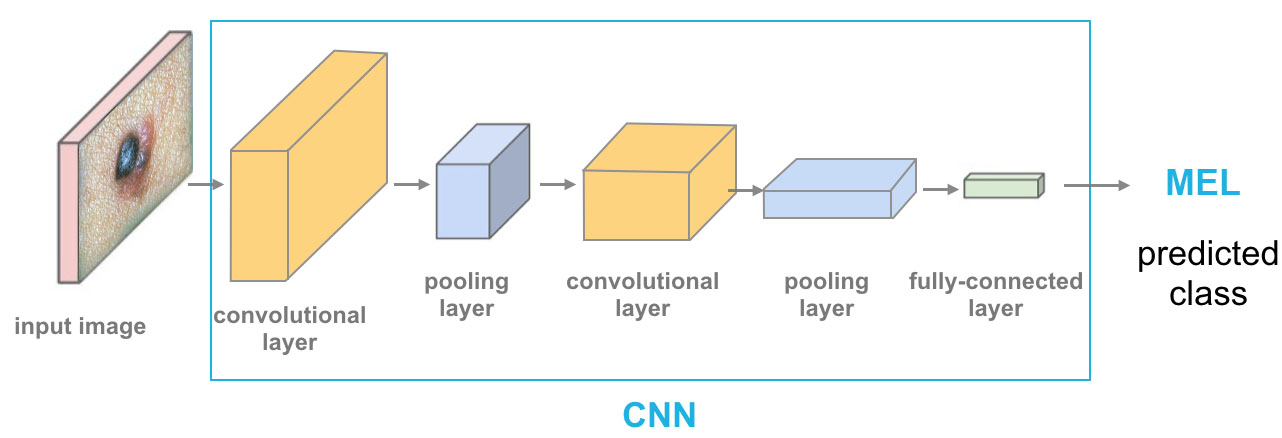
\includegraphics[width=0.9\linewidth]{images/CNN_ex.jpg}
    \caption{High level overview of CNN structures}
    \label{fig:CNN}
\end{figure}
\begin{figure}[hb]
    \centering
        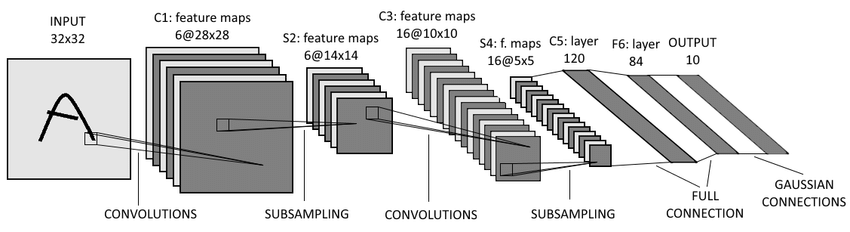
\includegraphics[width=0.7\linewidth]{images/deepLearning/leNet.png}
    \caption{LeNet-5 architecture \cite{LeNet} }
    
    \label{fig:LeNet}
\end{figure}
Image Classification is mostly achieved by using \textbf{Convolutional neural networks} (CNNs), a powerful way to learn useful representations of images and other un-structured data.\\
The name “convolutional neural network” indicates that the network employs a mathematical operation called convolution. Convolution is a specialized kind of linear operation. Convolutional networks are simply neural networks that use convolution in place of general matrix multiplication in at least one of their layers\cite{goodfellow}. A common example of a CNN architecture for image classification is shown in Figure~\ref{fig:CNN}. CNNs are a supervised learning method that learn the relationship between the input objects and the class labels and comprise two components: the hidden layers in which the features are extracted and, at the end of the processing, the fully connected layers that are used for the actual classification task. \\
In the context of image classification, a CNN in general does not process the input as a single block but as a composition of features. Unlike a common DNN, a CNN uses Fully-Connected layers only in the final part to produce the output, the classification probability distribution. 
\subsubsection{Architecture}
Figure~\ref{fig:CNN} shows an high-level structure of a CNN. Apart from the input layer, the middle layers achieve feature extraction while the final fully connected part performs classification.
Generally, feature extraction is performed by a repeated pattern. A convolutional layer is applied to the input,and then an activation function
and finally a Pooling layer, which reduces the information size.
An example of one of the first CNN created is shown in figure \ref{fig:LeNet}.
Unlike fully connected layers, convolution layers perform a convolution. The weights in a convolutional network are grouped into arrays called kernels.
Although they have a smaller width and height than the entrance, in basic CNN architectures they must match the depth.
Consider the input layer, an image usually has 3 dimensions: width, height and depth (in addition RGB encoding). So the first set of kernels must have a depth of three.\\
\begin{figure}[]
    \centering
        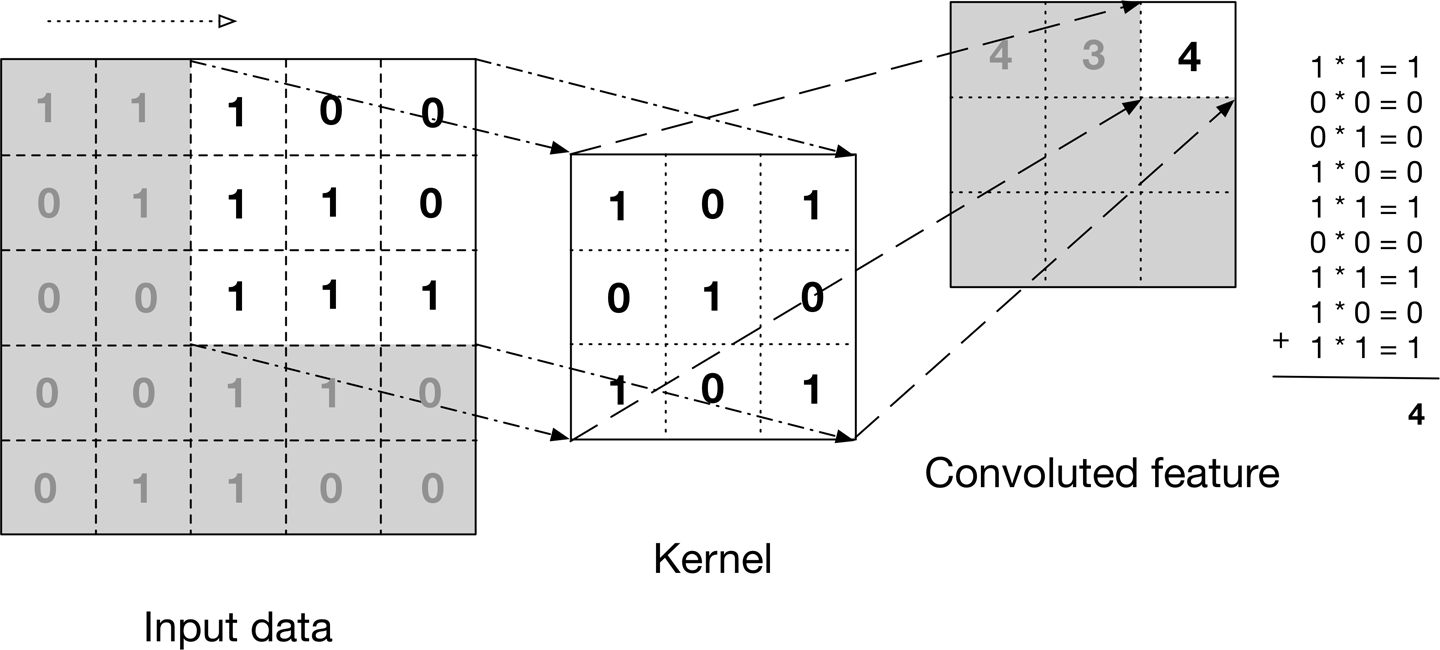
\includegraphics[width=0.7\linewidth]{images/deepLearning/conv.png}
    \caption{Convolution \cite{DeepLearningApproach} }
    \label{fig:Convolution }
\end{figure}
As shown in figure \ref{fig:Convolution  }, the convolution operation is applied by multiplying a kernel by an area in the input image. The result is then stored in the output matrix called feautere map. Once the input has been processed, the network uses the following kernel.\\
The \textbf{Pooling layer} combines similar features found in the feature map and helps prevent overfitting. The most common layer is Max Pooling, which extracts the maximum value.
Figure~\ref{fig:MaxPool } shows an example of Max Pooling with a stride of two.\\
\begin{figure}[]
    \centering
        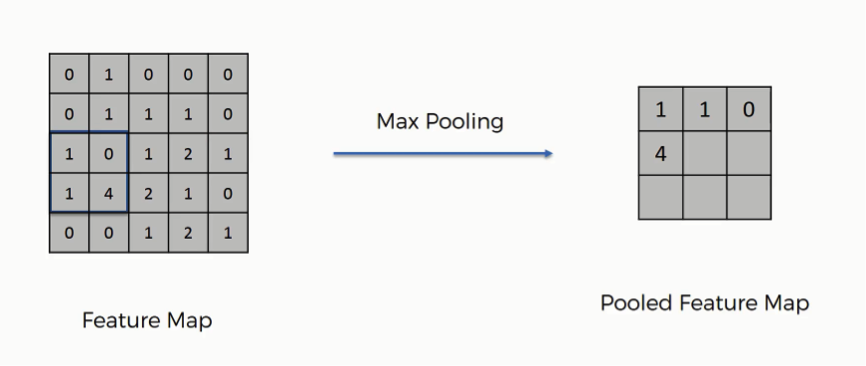
\includegraphics[width=0.7\linewidth]{images/deepLearning/maxpool.png}

    \caption{Max Pooling \cite{MaxPoolImage} }
    \label{fig:MaxPool }
\end{figure}
The \textbf{fully connected} layer takes the convolution or pooling output, flattens it and predicts the label that is most suitable for the input.
\subsection{Multi-task learning}
Recent works demonstrated that neural network also perform well in \textbf{multi-task learning}(MTL), that is the field, which takes care of learning more than one task at a time.
This approach showed that what is learned for each task can help other tasks be learned better.
In \cite{MTL}, performance of single task learning(STL) and MTL were compared; the related work showed that the extra information given in the MTL allowed to obtain better result than STL, especially in a real domain with medical background.\\
Sebastian Ruder in \cite{MTLoverview} presented two main MTL methods, shown in Figure~\ref{fig:MTLparadigms}, for Deep Learning: 
\begin{enumerate}[label=\Alph*]
\item Hard parameter sharing: this approach consists in sharing the hidden layers between all tasks, while keeping several task-specific output layers.
\item Soft parameter sharing: in this approach each task has its own model with its own parameters.
\end{enumerate}
Depending on the proposed strategy, a constraint is introduced among the parameters of the model.


\begin{figure}
    \centering
    \begin{subfigure}[b]{0.42\linewidth}        %% or \columnwidth
        \centering
        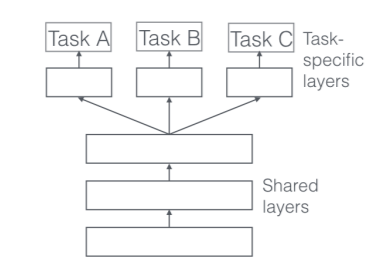
\includegraphics[width=\linewidth]{images/mtl hard.png}
        \caption{Hard parameter sharing approach}
        \label{fig:Hard}
    \end{subfigure}
    \begin{subfigure}[b]{0.54\linewidth}        %% or \columnwidth
        \centering
        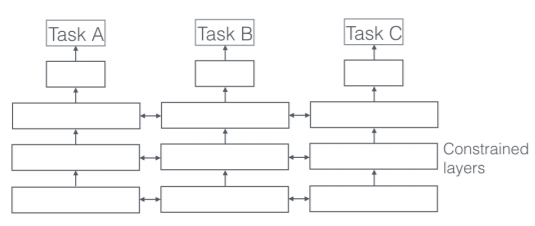
\includegraphics[width=\linewidth]{images/mtl soft.png}
        
        \caption{Soft parameter sharing approach}
        \label{fig:Soft}
    \end{subfigure}
    \caption{MTL sharing paradigms \cite{MTLoverview}}

    \label{fig:MTLparadigms}
\end{figure}

As shown in \cite{MTLoverview}, MTL performs well and it improves the learning process; it shows the following properties:
\begin{enumerate}
\item Implicit data augmentation: learning multiple tasks at the same time, permits to average the noise and provide a good representation for all the tasks.
\item Attention focusing: Sometimes differentiating relevant and irrelevant features for learning a task could be difficult due to noisy or limited data; MTL can help the model focus its attention on those features that actually matter as other tasks will provide additional evidence for the relevance or irrelevance of those features
\item Eavesdropping: learning some features for one task A could be more difficult than for a task B; learning them together allows task B to learn these features through B.
\item Representation bias: the representation of data will be generalized to provide a general structure to perform well with multiple tasks.
\item Regularization: by introducing an inductive bias, MTL reduces the risk of overfitting.
\end{enumerate}



\section{ML applications to skin lesion diagnosis}
Skin cancer detection and classification is a hot research topic since 1990's, and in literature many works were proposed \cite{7ptCNNforMel,estevaMLinDerm,mtl7ptCoppola,Kawahara,MLinDermat,HanWork}
Machine learning algorithms have the potential to improve the dermatologist’s practice from diagnosis to personalized treatment \cite{MLinDermat}. 
Supervised learning is the most common type of learning used in dermatology \cite{MLinDermat}.
A significant research regarding skin lesion classification is represented by the work of Esteva et al.~\cite{estevaMLinDerm}, that collected 129450 macroscopic images consisting of 2032 diseases. A Deep Neural Network (DNN) was trained on an Inception-V3 architecture using transfer learning, with weights pre-trained on ImageNet~\cite{ImageNet}. The prediction performances were tested against dermatologists on biopsy-proven clinical images.
Han et al.~\cite{HanWork} have merged different public datasets with a proprietary dataset to gather over 20.000 samples of macroscopic images, with 12 classified diseases. The ResNet \cite{Resnet} network architecture with weights pre-trained on ImageNet was used for this approach. Transfer learning was performed by freezing the weights of lower-level layers, in order to preserve the basic feature extraction from images.
The interest in skin lesion diagnosis using dermoscopic images increased after the ISIC dataset challenge was introduced \cite{IsicChallenge}, alongside with the benchmark for evaluation. The best performing approach was obtained by using an ensemble of DNNs and enhancing the number of samples by merging other datasets\cite{multiDataset}. \\
There are also methods developed upon both types of images and including additional metadata, working on the derm7pt dataset \cite{Kawahara}, which includes information for the 7 attributes used in the 7-point checklist diagnosis method.
Kawahara et al.\cite{Kawahara} developed a model for diagnosis prediction by joining two InceptionV3 networks with pre-trained weights on ImageNet \cite{ImageNet}. Since the 7-point checklist and the diagnosis are related tasks, the results are improved due to the higher generalization of a multi-task model. Furthermore, the model performance is increased by combining the outputs of the complementary modalities. During training all the modalities are available, whereas for the inference stage one or a specific combination of modalities can be used.
In Coppola et al.~\cite{mtl7ptCoppola} a MTL application was proposed. The authors of this work implemented a MTL method that learns what to share between tasks through gates, which allows the inspection of the relationships learned by the network. By means of gate blocks they allow tasks to share useful features. \\ 
Alzahrani et al.~\cite{7ptCNNforMel} developed a method for skin lesion detection and melanoma diagnosis from dermoscopy images by combining seven-points checklist criteria with convolutional neural networks. The proposed models have been realised by incorporating automated lesion feature extraction achieved by multi-input CNN considering standardised images (dermoscopy) and non-standardised images (clinical). This methos is similar to a concept bottleneck model, in which it first predicts the 7-point checklist attributes, and then use them for melanoma diagnosis, by applying 7-point algorithm.

 
